% ===== Figure & table includes for the TCI paper (generated 2026-09-30) =====
% Requires: \usepackage{graphicx}, \usepackage{booktabs}

% === Fig 1: hero triptych (double column) ===
\begin{figure*}[t]
    \centering
    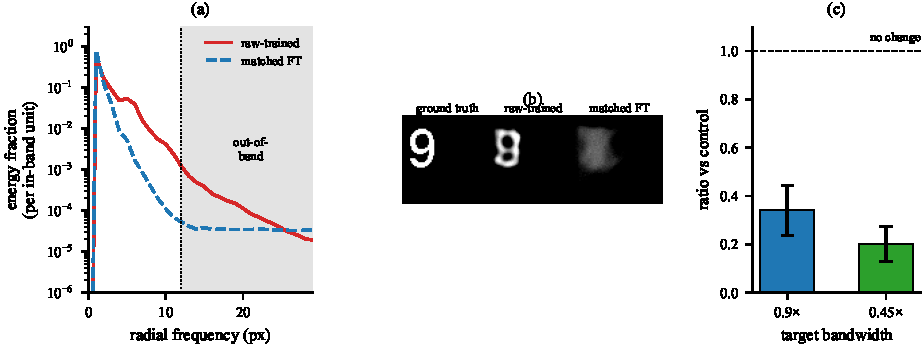
\includegraphics[width=0.95\textwidth]{figures/fig1_hero.pdf}
    \caption{Training-target bandwidth controls spectral fabrication. (a) Out-of-band energy is the reconstruction spectral energy outside the measured MTF support (shaded, vertical dotted line at the support radius); from an identical initialization, the raw-trained model keeps substantially more energy in this region (3$\times$ at the band edge) than the model fine-tuned against bandwidth-matched targets. (b) Reconstructions: the bandwidth-matched model suppresses out-of-band fabrication at the cost of visibly smoother (band-limited) output, which is the correct behavior under the measured information support; the raw-trained model restores sharper structure partly by inventing out-of-band content. (c) Suppression ratio of fine-tuned to compute-matched control out-of-band energy across both architectures and all seeds. Out-of-band energy is a fabrication proxy, not a perceptual metric.}
    \label{fig:hero}
\end{figure*}

% === Fig 2: paired control (single column) ===
\begin{figure}[t]
    \centering
    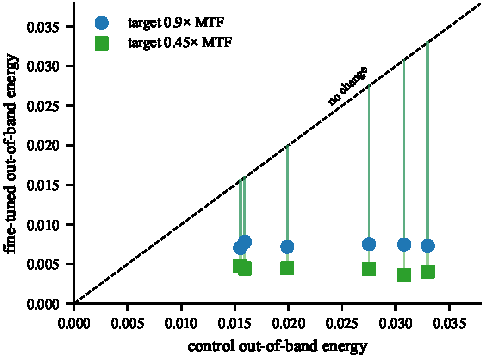
\includegraphics[width=0.48\textwidth]{figures/fig2_paired_control.pdf}
    \caption{Paired fine-tune versus compute-matched control (identical initialization; equal extra optimization). Each segment connects a unit's control value (on the no-change line) to its fine-tuned value. Matched-target ratio $0.34\pm0.11$ and half-target $0.20\pm0.08$; all 6/6 units reduce (one-sided sign test $p\approx0.016$).}
    \label{fig:paired}
\end{figure}

% === Fig 3: capacity (single column) ===
\begin{figure}[t]
    \centering
    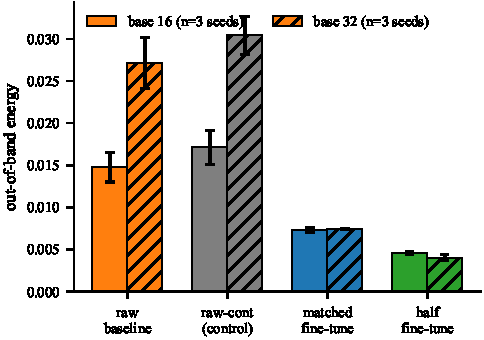
\includegraphics[width=0.48\textwidth]{figures/fig3_capacity.pdf}
    \caption{Out-of-band energy by arm for the two tested capacities. In the two tested capacities, the larger network fabricates more in the raw-baseline and control arms and admits stronger suppression under bandwidth-matched fine-tuning; described as an observed trend, not a scaling law. Error bars: std over 3 seeds.}
    \label{fig:capacity}
\end{figure}

% === Fig 4: trade-off (single column) ===
\begin{figure}[t]
    \centering
    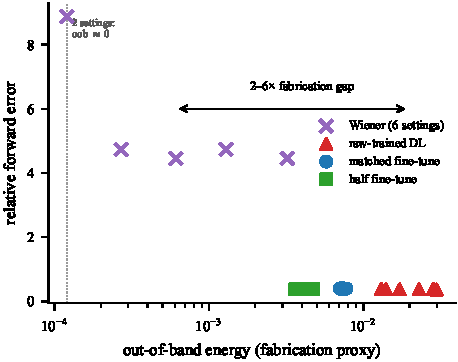
\includegraphics[width=0.48\textwidth]{figures/fig4_tradeoff.pdf}
    \caption{Fabrication versus forward fidelity. Wiener reconstructions (6 regularization/support settings) constrain out-of-band energy below the raw-target and matched arms in every cell (the half-bandwidth arm approaches the Wiener range) but operate at a roughly $1.4\times$ (${\sim}40\%$) worse relative forward error --- the learned arms therefore occupy a distinct operating point rather than dominating. Two Wiener settings with negligible out-of-band energy are drawn at the axis floor.}
    \label{fig:tradeoff}
\end{figure}

% === Fig 5: robustness (double column) ===
\begin{figure*}[t]
    \centering
    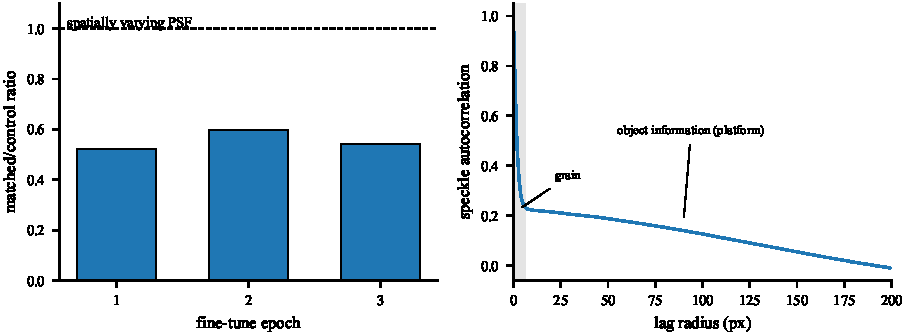
\includegraphics[width=0.92\textwidth]{figures/fig5_robustness.pdf}
    \caption{Left: the matched/control out-of-band ratio under a position-dependent (spatially varying PSF) forward operator remains stable across fine-tune epochs --- the suppression effect does not rely on shift-invariance. Right: measured speckle autocorrelation from the public experimental dataset (DSC): a sub-pixel grain peak superposed on a wide platform that carries object information out to $\sim$190\,px lag --- the real-data structure our protocol targets; quantitative real-data reconstruction is left to future work (see text).}
    \label{fig:robustness}
\end{figure*}

% === Table 1 ===
\begin{table}[t]
\centering
\small
\caption{Out-of-band energy (fabrication proxy) and band-limited PSNR across arms; mean$\pm$std over 6 units (2 architectures $\times$ 3 seeds). The paired block reports fine-tune-to-control ratios within units.}
\label{tab:main}
\begin{tabular}{lcc}
\toprule
Arm & Out-of-band energy & PSNR (dB) \\
\midrule
Raw baseline (20 ep) & $0.0210 \pm 0.0073$ & $16.5 \pm 0.4$ \\
Bandwidth-matched baseline (20 ep) & $0.0066 \pm 0.0006$ & $31.7 \pm 1.3$ \\
Half-bandwidth baseline (20 ep) & $0.0036 \pm 0.0004$ & $22.1 \pm 1.2$ \\
Raw-continued control (+4 ep) & $0.0238 \pm 0.0077$ & $16.4 \pm 0.5$ \\
Matched fine-tune (4 ep) & $0.0074 \pm 0.0003$ & $29.8 \pm 0.9$ \\
Half fine-tune (4 ep) & $0.0043 \pm 0.0004$ & $21.8 \pm 0.2$ \\
\midrule
\multicolumn{3}{l}{Paired (fine-tune vs.\ control, within unit)} \\
Matched fine-tune ratio & $0.34 \pm 0.11$ & reduced 6/6 \\
Half fine-tune ratio & $0.20 \pm 0.08$ & reduced 6/6 \\
\bottomrule
\end{tabular}
\end{table}

